\chapter{Sistem de dialog}

% todo: citari de sericii si lucrari

Construcția unui agent virtual menit să întrețină cursul unei conversații a fost întotdeauna un etalon al performanței de cercetare, de aceea testul ce poartă numele cercetătorului britanic Allan Turing \ref{test-turing} a fost pană de curând un criteriu în această direcție.

Au fost propuse diferite arhitecturi și moduri de a schița matematic o conversație, printre ele și ELIZA compus dintr-un set de reguli elaborate pe baza mai multor studii având la bază logica. Bineînțeles industria cere și abordări mai modulare, mai robuste dar care să nu iasă din tipare, în această speță făcându-și apariția prima arhitectură bazată pe umplerea de sloturi (GUS), adică pentru fiecare replică din dialog se extrag constituenți semantici specifici domeniului care mai apoi sunt completați într-o structură tabelară (frame) urmând să servească drept parametrii în interogările cu sistemul.

Dacă privim la scopul final al unei conversații distingem două clase și anume: agenți orientați pe rezolvarea de cerințe și agenți orientați pe discuție la nivel general.

Cum majoritatea asistenților virtuali sunt dezvoltați în scopuri comerciale, rezolvarea cerințelor primează în funcționalitatea unei astfel de aplicații, așadar industria se concentrează pe arhitecturi modulare, care să necesite cât mai puține date de antrenare, RASA, SNIPS, WATSON, DialogFlow sunt platforme care pun la dispoziție instrumente pentru a crea genul acesta de agenți.

Prin natura sa, lumea academică este întotdeauna mai în față în ceea ce privește tehnica sa de a concepe aceste sisteme, mai exact se folosesc rețele neurale recurente pentru a capta contextul unei replici și pentru a genera răspunsuri, iar pentru contextul conversației și generarea unor politici de răspuns se folosește învățarea prin recompensă. \cite{rl-seq2seq}

În cadrul studiului curent accentul este pus pe structura ce îmbină mai multe modele, drept pentru care vor vi detaliate experimentele pentru NLU și DM.

\section{Înțelegerea limbajului natural}
NLU este un concept destul de vast, in terminologia sistemelor de dialog acesta joacă rolul componentei care detectează intenția vorbitorului si extrage constituenți semantici din limbajul natural exprimat.
Detecția intenției poate fi tratata ca o problema de clasificare a unei replici din punct de vedere semantic, iar recunoașterea entităților poate fi văzută ca o etichetare de secvențe.
\subsection{Abordări anterioare}

% todo: de citat lucrarile

Pentru detectarea intenției se pot folosi tehnici standard de clasificare a unui text si anume SVM (Haffner et al., 2003), dar si rețele neurale convoluționale (CNNs) (Xu and Sarikaya, 2013) întâlnite adesea în procesarea imaginilor.

Pentru recunoașterea entităților se folosesc abordări precum (MEMMs) (McCallum et al., 2000), conditional random fields (CRFs) (Raymond and Riccardi, 2007), și rețele neurale recurente (RNNs) (Yao et al., 2014; Mesnil et al., 2015)

Având la baza înțelegerea limbajului, majoritatea lucrărilor actuale se concentrează pe rezolvarea concomitenta a acestor doua probleme, întrucât combinarea celor doua modele ajuta la învățarea unei reprezentări cat mai precise a textului. \cite{joint models-attention models}


\subsection{Model propus}

Arhitectura matematică ce a devenit foarte populară în procesarea limbajului natural este rețeaua neurală recurentă, datorită formelor sale (LSTM/GRU) optimizate pentru învățarea automată ea se bucură de un succes răsunător. Aceste tipuri de rețele sunt folosite adesea ca structuri de bază pentru a crea alte modele de calcul, un exemplu este rețeaua de codificare-decodificare (seq2seq), formată din două rețele recurente, una pentru captarea (codarea) înțelesului unei secvențe iar cealaltă pentru operația de decodificare într-o secvență de ieșire.

Ambele probleme sunt rezolvate simultan folosind un codificator pentru reprezentarea înțelesului unei propoziții și două decodificatoare câte unul pentru fiecare chestiune.

\begin{figure}[htbp]
	\centering
	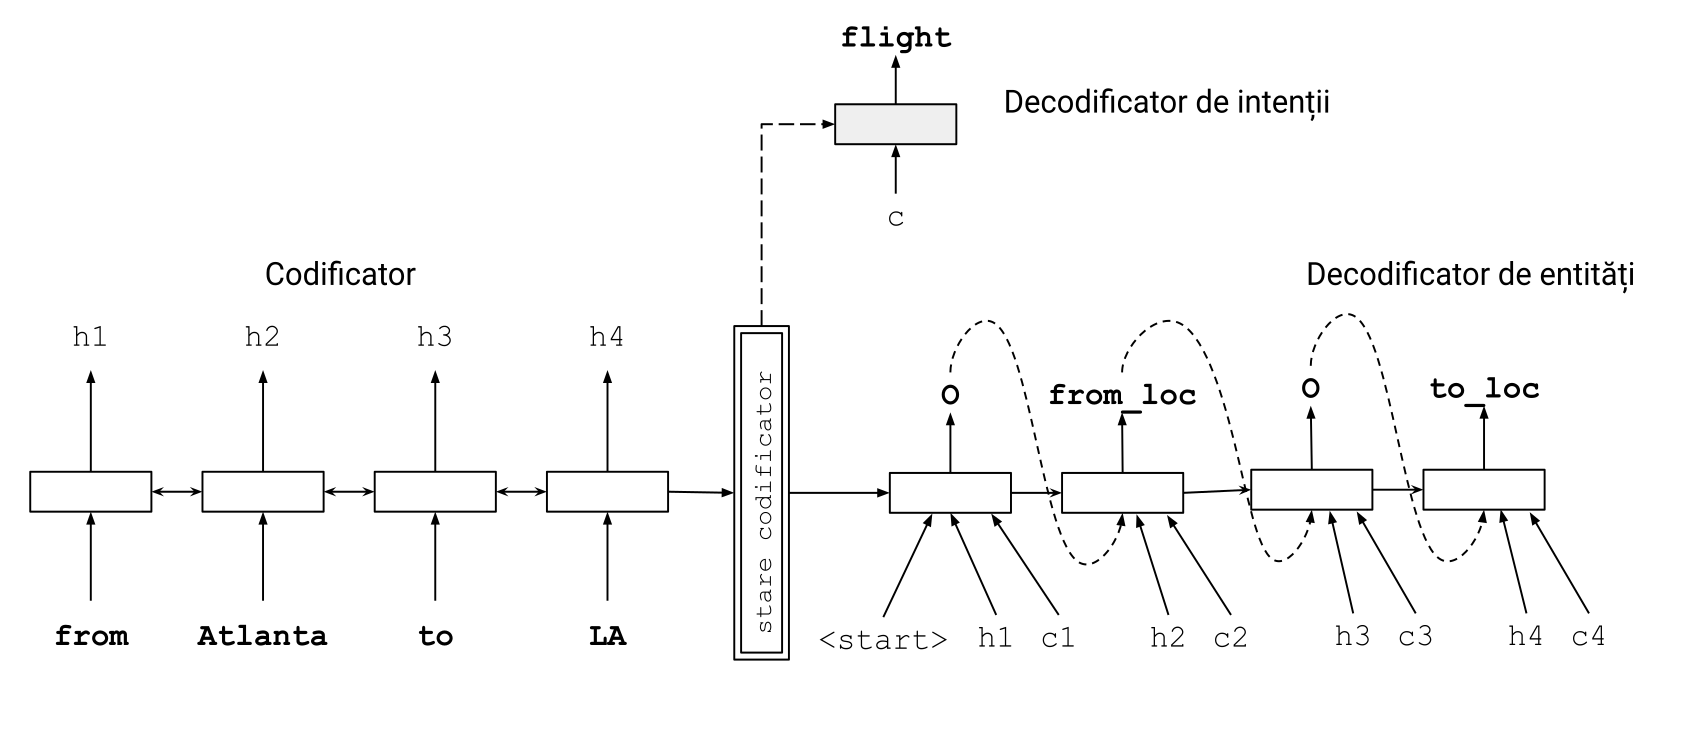
\includegraphics[scale=0.5]{seq2seq_x.png}
	\caption{Seq2Seq-x}
	\label{fig:enc_module}
\end{figure}

Pentru recunoașterea entităților se dorește etichetarea unei secvențe de cuvinte $ x= (x_1, ..., X_T)$ într-o altă secvență de nume de entități corespunzătoare $ y=(y_1, ..., y_T) $. Operația de codificare se realizează prin citirea întregii secvențe de către o rețea recurentă bidirecțională, adică

\begin{figure}[h]
	\centering
	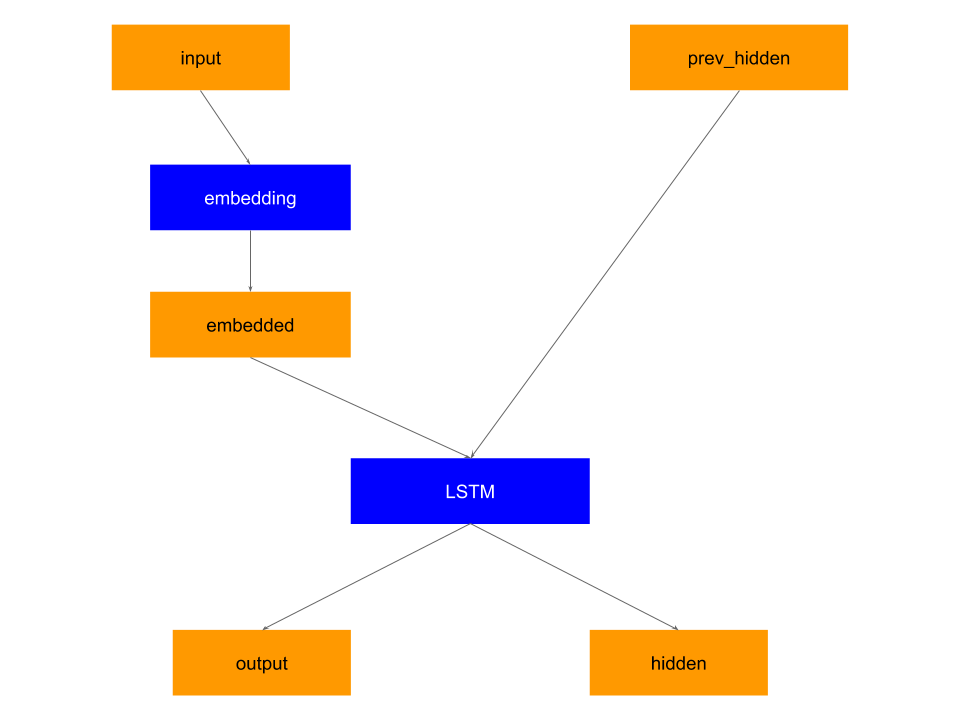
\includegraphics[scale=0.35]{encoder_module.png}
	\caption{Bidirectional Encoder}
	\label{fig:enc_module}
\end{figure}


\begin{figure}[h]
	\centering
	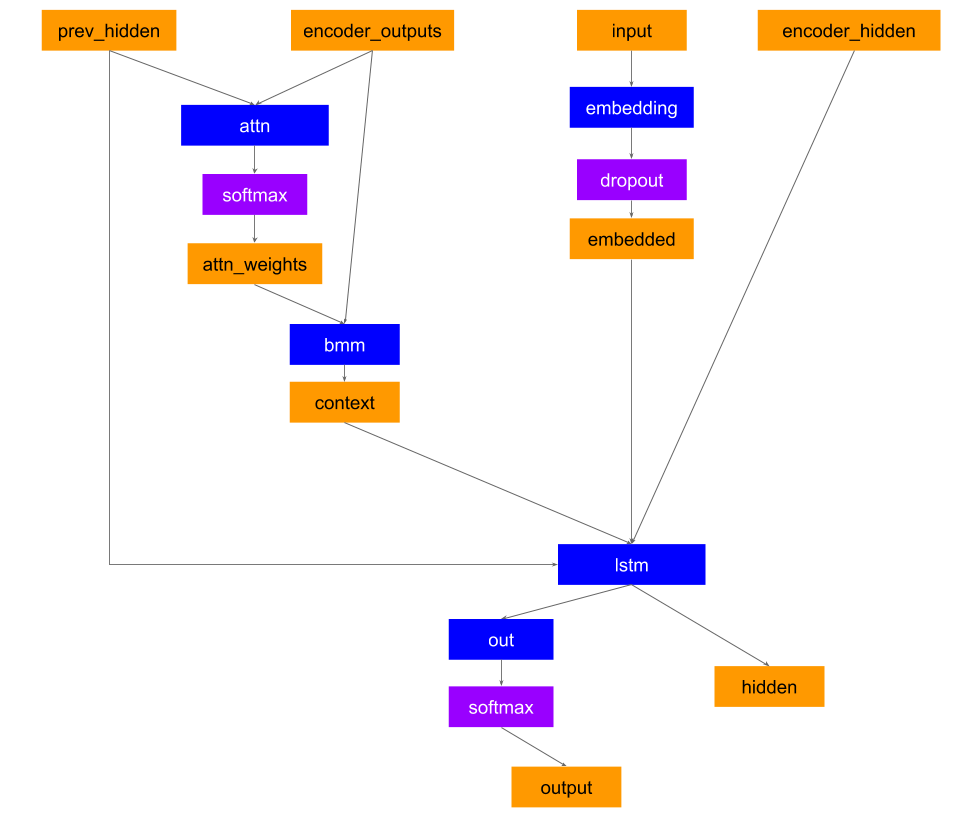
\includegraphics[scale=0.35]{decoder_bahdanau.png}
	\caption{Attention Decoder}
	\label{fig:dec_bah}
\end{figure}

\section{Administrator de dialog}

\subsection{Abordări anterioare}

\subsection{Slot filling}

\section{Metode de evaluare}

\section{Rezultate}